\section{Using native reduction when symbolic algebra costs more}
\label{sec:notes-parser-guard}
The symbolic regressions motivate a narrower use of the new recurrence. Before entering it, the final application checks whether all masses and scalar products are direct rational values. If an input requires symbolic parsing, the application keeps the older exact formulas where they apply and otherwise uses Kira. This rule leaves the learned models and the existing native settings unchanged. It controls the cost of the new analytic stage; it does not estimate a reduction coefficient.

Two development requests use the massive symbolic two-point family with powers $(4,1)$ and $(1,4)$. We enable the rule only when it reduces their summed median time by at least five percent. The reserved comparison then uses powers $(3,2)$ and $(2,3)$, two independent products containing those blocks at loop orders two and thirteen, and five compatibility requests. Appendix~\ref{app:notes-parser-guard} specifies these inputs. Each method runs three times in a fresh process, and all four methods pass every exact coefficient comparison.

\begin{table}[!htbp]\centering\small
\caption{Separate validation of the final input rule. Times are sums of per-request medians in seconds. The initial analytic variant has the new recurrence but lacks the input rule. Native and fixed controls retain the same prepared master indices and factorization.}
\label{tab:notes-parser-guard}
\begin{tabular}{@{}lrrrrr@{}}\toprule
Collection & $N$ & Final & Initial analytic & Native & Fixed\\\midrule
Symbolic inputs & 4 & 3.333 & 23.145 & 3.442 & 3.461 \\
Compatibility & 5 & 7.919 & 7.835 & 10.930 & 8.294 \\
All requests & 9 & 11.252 & 30.980 & 14.371 & 11.755 \\
\bottomrule\end{tabular}\end{table}

For the four symbolic requests, the final method uses 85.6\% less time than the initial analytic variant. Its time ratio is 0.144, with repetition interval $[0.098,0.159]$.

For the five compatibility requests, the final method uses 1.1\% more time than the initial analytic variant. Its time ratio is 1.011, with repetition interval $[0.965,1.105]$. The interval includes equal times.

For all nine requests, the final method uses 63.7\% less time than the initial analytic variant. Its time ratio is 0.363, with repetition interval $[0.269,0.392]$.

Across all nine requests, the final method uses 21.7\% less time than the matched native control, with time ratio 0.783 and repetition interval $[0.734,0.853]$. Against the fixed control, the ratio is 0.957, with interval $[0.913,1.040]$. This interval includes equal times, so this follow-up does not establish an additional learned saving. The symbolic subset uses the same native branch in both final and native methods; its small timing difference also has an interval that includes one.

All 9 requests complete in every repetition, giving 108 timed reductions and 3,084 exact coefficient comparisons. Independent reference preparation takes 47.230 seconds and remains separate. The first-attempt total for the final method is 12.048 seconds; this total includes every requested input.

\begin{figure}[!htbp]\centering
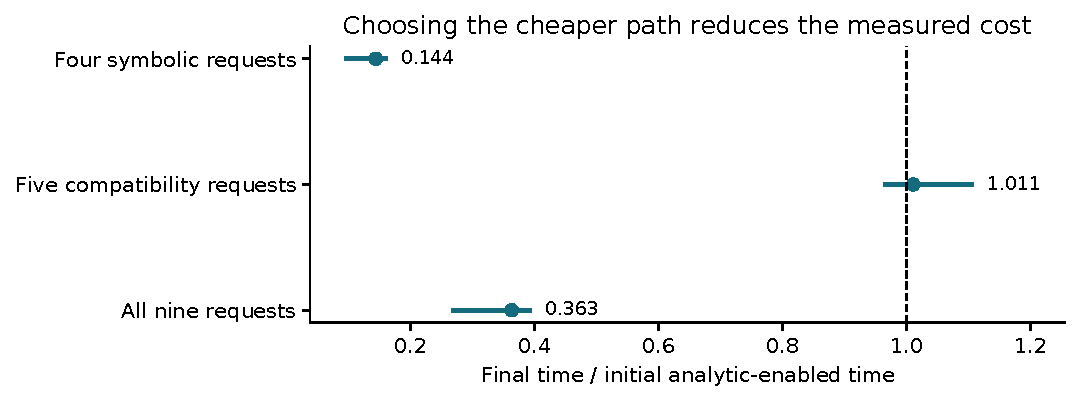
\includegraphics[width=.9\linewidth]{paper_figures/parser_guard.pdf}
\caption{The input rule bypasses symbolic recurrence work where native reduction is cheaper. Values below one favor the final rule. Intervals resample three repetitions on these fixed inputs. Compatibility requests check that other application branches remain available.}
\label{fig:notes-parser-guard}
\end{figure}

The final rule uses native Kira for the four symbolic requests, so their saving relative to the initial analytic variant is an integration improvement. This test compares complete paths and does not separately measure parsing, import, and symbolic arithmetic costs. It is not an additional ML contribution. The earlier 41-request experiment and this nine-request test use different targets and remain separate comparisons. We do not combine their times into a new overall speedup or claim that every symbolic family benefits from this rule.
